\subsection{Формула Эйлера}

\begin{theorem}[Формула Эйлера, 1758]~

    Во всяком связном плоском графе выполняется равенство $|V| - |E| + |F| = 2$.
    
\end{theorem}

\begin{proof} 
    Индукция по числу граней.

    \textsl{База:} $|F| = 1$ --- это дерево, равенство $|V| - |E| = 1$ выполняется по теореме о деревьях.

    Пусть $|F| \geq 2$. Удаляем одно ребро, входящее в цикл; оно разделяло две грани.

    Получается граф, в котором $|V|$ вершин, $|E| - 1$ ребер, $|F| - 1$ граней.

    Для него, по предположению индукции, выполняется $|V| - (|E| - 1) + (|F| - 1) = 2$,
    откуда следует $|V| - |E| + |F| = 2$.\\

\end{proof}

\begin{follow}
    Число граней в планарном графе не зависит от его укладки.
\end{follow}


\begin{center}
    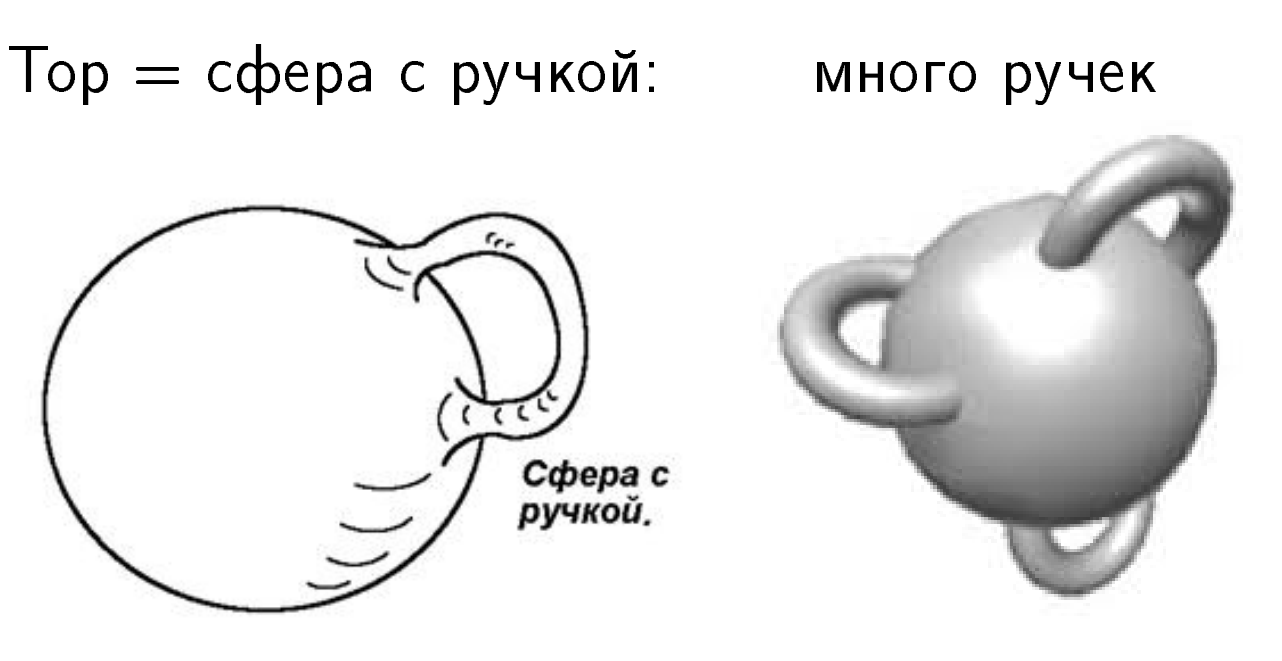
\includegraphics[width=0.4\textwidth]{par26tor.png}
\end{center}

\begin{theorem}[обобщение формулы Эйлера]~
    
    Для графа, укладываемого на тор с $k$ ручками, выполняется $|V| - |E| + |F| = 2 - 2k$.

    В укладке граф связный, каждая грань является областью, то есть гомеоморфна диску.

    Без доказательств и без формальных определений.

\end{theorem}

\begin{center}
    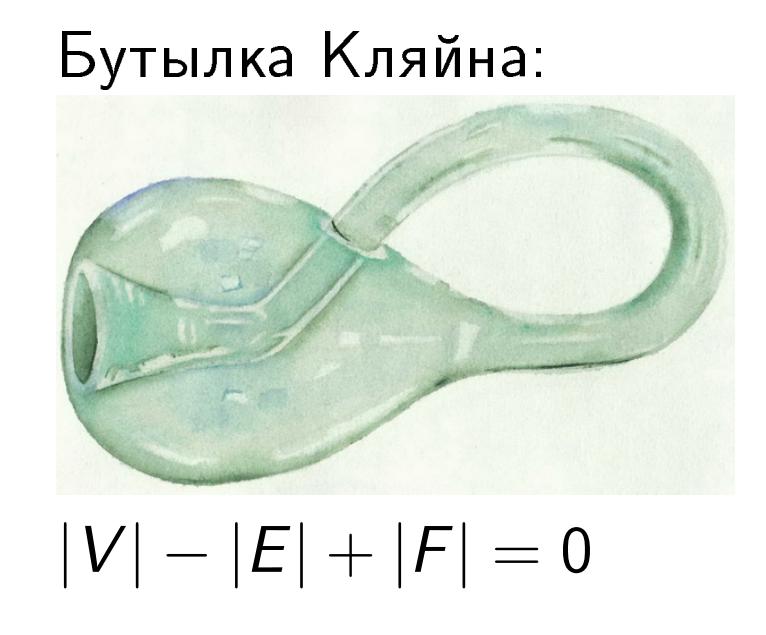
\includegraphics[width=0.4\textwidth]{par26klain.png}
\end{center}

\begin{theorem}
    \label{thm:3v6e}
    
    Во всяком планарном графе $G = (V, E)$ без петель и кратных ребер, где $|V| \geq 3$, выполняется неравенство $|E| \leq 3|V| - 6$.

    Если, кроме того, всякий цикл в графе имеет длину не менее чем $l$, то $|E| \leq \frac{l}{l - 2} (|V| - 2)$.

\end{theorem}

\begin{proof}
    Граф допускает укладку с некоторым множеством граней $F$.
    
    Утверждение: Длина границы каждой грани не менее чем $3$.

    Если длина границы $2$, то имеем цикл длины $2$, то есть кратное ребро --- а по условию их нет. Если длина границы $1$, то имеем петлю.

    Грани соответствует как минимум три ребра, а ребру соответствует не более двух граней, получаем $3|F| \leq 2|E|$.

    Подставим в формулу Эйлера $|V| - |E| + |F| = 2$:


    \begin{gather*}
        3|V| - 3|E| + 2|E| \geq 3|V| - 3|E| + 3|F| = 6 \\
        \implies |E| \leq 3|V| - 6.
    \end{gather*}

    Вторая часть: здесь $l|F| \leq 2|E|$, и далее из формулы Эйлера $l|V| - l|E| + 2|E| \geq l|V| - l|E| + l|F| = 2l$, откуда следует требуемое неравенство.

    \begin{gather*}
        l|V| - l|E| + 2|E| \geq 2l \implies l|V| - (l - 2)|E| \geq 2l \implies l|V| \geq (l - 2)|E| + 2l\\
        \implies |E| \leq \frac{l}{l - 2}(|V| - 2) 
    \end{gather*}
\end{proof}

\begin{follow}
    Во всяком планарном графе $G = (V, E)$ без петель и кратных ребер есть вершина степени не более чем $5$.
\end{follow}

\begin{proof}
    Пусть все вершины имеют степень $6$ и более. Тогда 

    \[ \sum\limits_{v \in V} \deg v \geq 6|V|. \]

    С другой стороны,

    \[ \sum\limits_{v \in V} \deg v = 2|E|. \]

    Отсюда вытекает, что $|E| \geq 3|V|$. Противоречие с $|E| \leq 3|V| - 6$.

\end{proof}